

\subsection{Program Structure}
\label{sec:ProgramStructure}

Now when the operating system is defined, the next stage will be to define the actual application that needs to be implemented. Given the block diagram of figure \ref{fig:TheSystemBlockDiagram}, the blocks that make up the system is already defined.

\subsubsection{Defining tasks}
\label{sec:DefiningTasks}
First step is to identify the tasks that make up the system. A good rule of thumb is to make a driver task for every peace of hardware that the system is to interact with. This idea is based on the Parallel criteria which implies that things can be separated in to different tasks if the functionality runs independent and simultaneously, which indeed will be the case for a hardware driver. 
However the UART0 driver that supports connection between the PC and micro controller, can send and receive data independently. Therefore this task is split up in to two tasks. A receive task, and a transmit task.
Doing so also have the advantage of reusability, for other applications requiring the same hardware. 

Now when all the hardware is taken care of, the only thing remaining is the application it self. The application should be able to handle commands given by the user. Commands could be "set coordinate pan, tilt", "run light-show \#2" an "set minimum velocity tilt". Since the entire application will consist of function calls, the main body of the application will take the shape of a kernel task that execytes the functions defined in the function list shown in appendix 
%\ref{sec:}. 


By letting the primary source of user input be a terminal on an extern PC, the most natural application 
This gives the 

 The over all structure plan of the system is to make the 

feachures that should be supported 


Given the above mentioned requirements, a task diagram for the system was created, here the program were to handle two different sources of user input, in a manner that would not effect the application. 

\begin{figure}
	\centering
	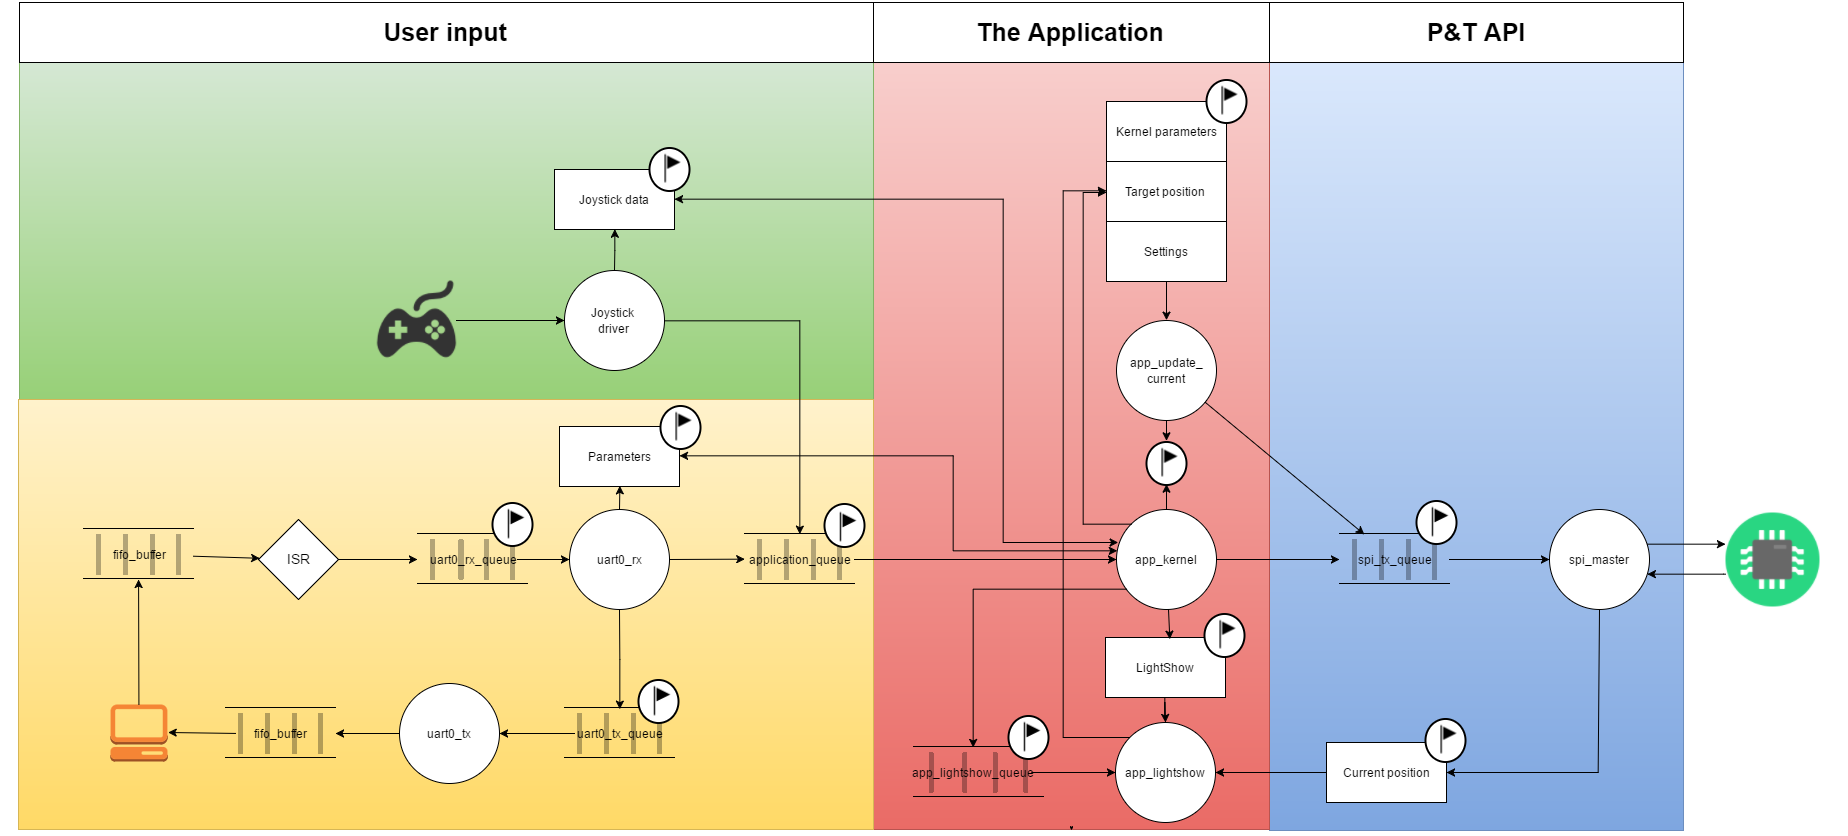
\includegraphics[scale= 0.4, angle = 90] {Billeder/microcontroller-Task-Diagram}
	\caption{The application task diagram}
	\label{fig:applicaiton_task_diagram}
\end{figure}


one task one input queue

now add the used semaphores at critical sections

Now when the task diagram has been made, it is time to considerer possible structural weakness such as deadlocks and handling og queues. 

